\section{Radiative correction}
The born process illustrated in Fig.~\ref{fig:rad} a) is not the only process
contributing to the measured pion electro-production cross section.
A photon or a $e^+e^- $ pair could be produced as well and the amplitudes
of these processes interfere with each other.
A {\em radiative correction} is necessary to extract the born process from the
measured cross section.

The  following radiative processes (in the lowest order of the
fine structure constant) are present in the measured events:
\begin{itemize}
\item the Bremsstrahlung, Fig.~\ref{fig:rad} b) and c) where a photon is emitted by
      the incoming or outgoing electron.
\item the vertex correction, Fig.~\ref{fig:rad} d), where a photon is emitted by the
      incoming electron and absorbed by the outgoing electron.
\item the vacuum polarization, Fig.~\ref{fig:rad} e), where the virtual photon
      produces temporarily an $e^+e^-$ pair.
\end{itemize}

\vspace{1cm}
\begin{figure}[h]
  \centering
                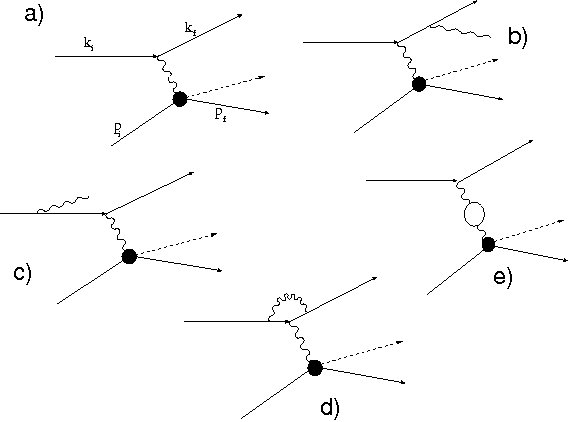
\includegraphics[width=0.85\textwidth ]{img/rad.jpg}
                \caption{ Feynman diagrams for the Born and radiative processes.
	             a) Born electro-production, b) and c) Bremsstrahlung d) vertex
		         correction, e) vacuum polarization.}
                \label{fig:rad}
\end{figure}

\clearpage\newpage
\subsection{The calculation of the radiative correction}
The radiative and acceptance corrections are tied to each other. In each bin, we have:
\begin{equation}\label{eq:cross_section}
	\sigma = \sigma_{MEAS}\times \textcolor{red} {(\frac{RAD_{GEN}}{RAD_{REC}})}
                         \times \textcolor{blue}{(\frac{NORAD_{GEN}}{RAD_{GEN}})}
\end{equation}
where:
\begin{itemize}
\item $\sigma_{MEAS}$ is the luminosity-normalized number of events with all the proper
factors, just before acceptance and radiative corrections.
\item $RAD_{GEN}$ is number of generated radiated events.
\item $RAD_{REC}$ is the number of reconstructed events after the MonteCarlo simulation,
reconstruction software and all the analysis cuts applied.
\item $NORAD_{GEN}$ is the number of generated non-radiated events.
\end{itemize}
$\textcolor{red}{RAD_{GEN} / RAD_{REC}}$ is the \textcolor{red}{acceptance correction} and
$\textcolor{blue}{NORAD_{GEN} / RAD_{GEN}}$ is the \textcolor{blue}{radiative correction}.

In an ideal situation when one could use a good model to calculate both the acceptance and
radiative corrections, the $RAD_{GEN}$ terms in Eq.~\eqref{eq:cross_section} are identical
and cancel each other out. One could say that the $RAD_{GEN}$ terms are dummy variables.

However it might happen\footnote{for example the software/model exists for one correction
only. This is the case for the exclurad software, which can only be used to calculate the
radiative correction and not to generate events.} that the $RAD_{GEN}$ terms are not
identical. In this case particular care should be taken to ensure they are as close
to each other as possible. The reason is simple to understand by looking at
Eq.~\eqref{eq:cross_section}: if the $RAD_{GEN}$ varies by a factor of two in
the acceptance correction, we want to radiative correction to reflect that,
or the cross section will be off also by a factor of two. One of the handles to
minimize the model dependance of the radiative correction and to bring the $RAD_{GEN}$
terms close to each other is the missing mass cut.

\subsection{The missing mass cut and the radiative correction}
When extracting the experimental cross section a missing mass cut
is applied to remove unwanted channels (double pion production, etc).

While it's clear that the same cut should be applied to the the $\textcolor{red}{RAD_{REC}}$,
there are two possible ways of applying the corrections in Eq.~\eqref{eq:cross_section}:
\begin{itemize}
 \item[a.] No missing mass cut is applied to the $RAD_{GEN}$ terms.
 \item[b.] A missing mass cut is applied to the $RAD_{GEN}$ terms.
\end{itemize}


In the radiative correction calculation the missing mass cut translates in how much energy the
radiated photon is allowed to take away from the outgoing hadronic system.
If no missing mass cut is applied, the calculation involves the integration of the
cross section from threshold to the $W$ bin considered. For high values of
$W$ this can be particularly dangerous, as various models may describe the $W$ spectra
quite differently. In Fig.~\ref{fig:vcut_0} an example of exclurad radiative correction
calculation is plotted as a function of $\phi^*$ for $W=1.77$ GeV and $Q^2=2.15$ GeV$^2$
with no restriction on missing mass cut for various models. As one
can see, there's a difference of $50\%$ in some bin.
In Fig.~\ref{fig:vcut_06} a calculation for the same bins is carried out, but
with $vcut=0.06$, corresponding, as shown in Eq.~\eqref{eq:vcut},
to a missing mass cut of $mm^2 = 0.0782$ $GeV^2$.

The preferred way to reduce the systematics coming from model dependance
is to apply a missing mass cut in the radiative correction calculation to
reduce the limits of integration. Furthermore, a missing mass cut will
bring the $RAD_{GEN}$ terms in Eq.~\eqref{eq:cross_section} close to each other.

\vspace{0.5cm}
\begin{figure}[h]
  \centering
                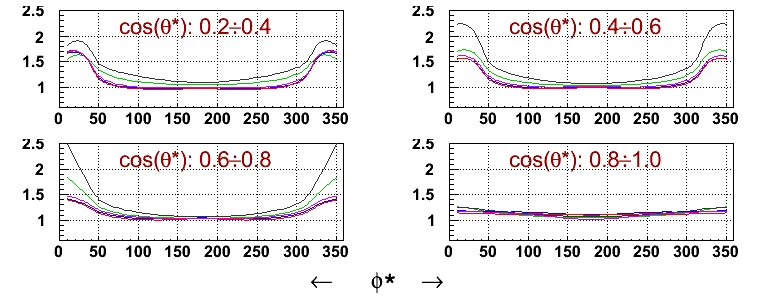
\includegraphics[width=0.90\textwidth ]{img/rad_cor_phi_vcut0.jpg}
                \caption{Radiative correction as a function of
	             $\phi^*$ for $W=1.77$ GeV and $Q^2=2.15$ GeV$^2$. Black: DMT2001.
                Green: MAID2002. Blue: MAID2003. Red: MAID2003 w/o the Roper Resonance.
                Violet:  MAID2007.
                No restriction on missing mass was applied (vcut = 0).
                The integration of the cross section starts from threshold,
                and calculations with different can differ by $50  \,^{\circ\!\!}/\!_\circ$}
                \label{fig:vcut_0}
\end{figure}


\vspace{0.5cm}
\begin{figure}[h]
  \centering
                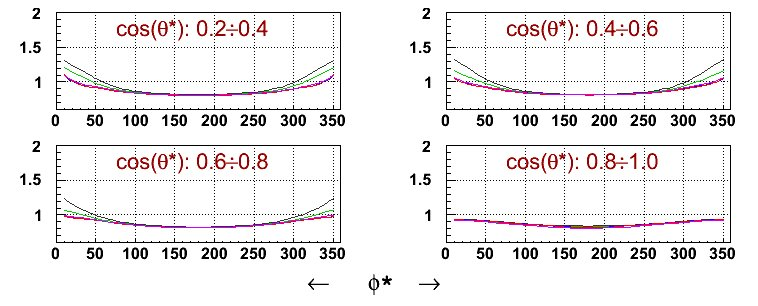
\includegraphics[width=0.90\textwidth ]{img/rad_cor_phi_vcut06.jpg}
                \caption{Radiative correction as a function of
	             $\phi^*$ for $W=1.77$ GeV and $Q^2=2.15$ GeV$^2$. Black: DMT2001.
                Green: MAID2002. Blue: MAID2003. Red: MAID2003 w/o the Roper Resonance.
                Violet:  MAID2007.
                No restriction on missing mass was applied (vcut = 0).
                The integration of the cross section starts from threshold,
                and calculations with different can differ by $50  \,^{\circ\!\!}/\!_\circ$}
                \label{fig:vcut_06}
\end{figure}



\clearpage\newpage
\subsection{Exclurad}
The radiative correction is calculated using the {\it exclurad} framework \cite{bib:radcorr},
which is based on a covariant method for infrared cancellation \cite{bib:radinfra}, is used.
Multiple soft photon radiation is included via exponentiation \cite{bib:shum}, \cite{bib:YFS}.
This method is preferred over the Mo and Tsai procedure \cite{bib:motsai} because:

\begin{itemize}
\item[1)] It addresses {\it exclusive} electroproduction rather than inclusive,
          involving all four un-polarized structure functions, as opposed to
          the Mo and Tsai formalism which accounts only for two structure functions
          and inclusive scattering and it is independent of outgoing hadron angles.
          In principle, the general formulas of Mo and Tsai can be adapted to the
          coincidence framework if the integration over the photon phase space is done properly.
\item[2)] The infrared cancellation is independent of the unphysical parameter $\Delta$
          separating the phase space of soft and hard photons necessary in the Mo and
          Tsai procedure and leading to uncertainties.
\item[3)] The approach of ref. \cite{bib:radcorr} does not rely on the peaking approximation,
          avoiding uncertainties at a few percent level associated with it.

\end{itemize}

The calculation of the radiative tail in this
framework separates the leptonic (the sole responsible for radiative effects)
and the hadronic currents. The structure functions $H_i$ are external to the
calculation of the radiative correction, can be thought as ``input'' and are provided
by theoretical models. 



The software {\it exclurad} \cite{bib:radcorr} has been developed to
calculate the radiative correction using as input for the hadronic current
various theoretical models (like MAID or DMT).
This program gives the radiative correction RC as the ratio
of the non-radiated to radiated four fold cross section:
$$
	RC(W, Q^2, \cos\theta^*, \phi^*) =\frac{\sigma_{RAD}}{\sigma_{NORAD}} = \textcolor{blue}{\frac{RAD_{GEN}}{NORAD_{GEN}}}
$$
In the e1-6 analysis we used {\it exclurad} for the radiative correction.
Fig.~\ref{fig:rad_cor_thetaphi_W_143_Q2_300maid2002} shows the correction as a function
of $\cos\theta^*$ and $\phi^*$ for $W=1.43$ GeV and $Q^2=3$ GeV$^2$ for the model maid2002.
See   \href{http://www.jlab.org/~ungaro/maureepage/proj/pi0/distributions/radiative_correction.html}
{radiative correction plots} for the correction in each bin considered as a function of $\phi^*$ or
$\cos\theta^*$ or both.

\begin{figure}[h]
  \centering
                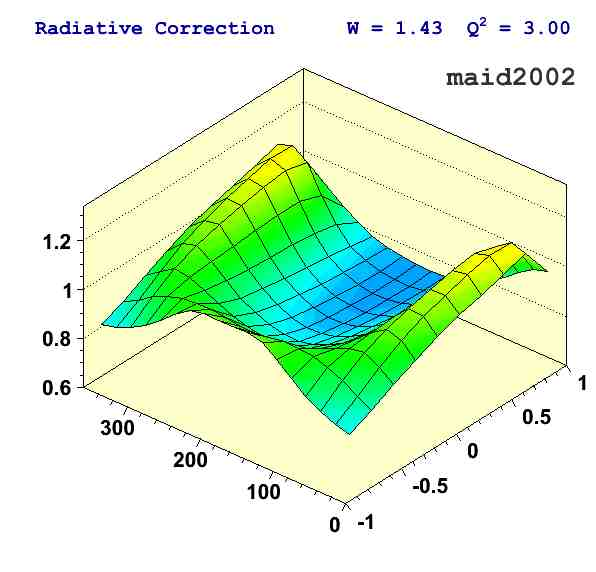
\includegraphics[width=0.75\textwidth ]{img/rad_cor_thetaphi_W_143_Q2_3maid2002.jpg}
                \caption{Radiative correction as a function of
	             $\cos\theta^*$ and $\phi^*$ for $W=1.43$ GeV and $Q^2=3$ GeV$^2$. The model used for
                this plot is maid2002.}
                \label{fig:rad_cor_thetaphi_W_143_Q2_300maid2002}
\end{figure}



\clearpage\newpage
\subsubsection{How to use exclurad}
The software {\it exclurad} can be downloaded from \href{http://www.jlab.org/RC/exclurad}{http://www.jlab.org/RC/exclurad}
or in the subversion repository with the following command:

\begin{verbatim}
     svn co  https://jlabsvn.jlab.org/svnroot/clas/trunk/analysis/exclurad
\end{verbatim}

{\it Exclurad} uses a file named ``input.dat'' to get the calculation parameters. An example is shown below:
\vspace{0.6cm}
\begin{verbatim}
3       !  1: AO 2: maid98  3: maid2000
0       !  0: Full, 1: Factorizable and Leading log (peaking appr)
5.754   !  bmom - lepton momentum
0.0     !  tmom - momentum per nucleon
1       !  lepton - 1 electron, 2 muon
1       !  ivec - detected hadron (1) p, (2) pi+
0.06    !  vcut - cut on v. (0.) if no cut, negative -- v

3

2.800 2.800 2.800
2.000 2.000 2.000
0.800 0.800 0.800
10.00 90.00 150.0
\end{verbatim}\vspace{0.6cm}
{\bf vcut} is defined as:
\begin{equation}\label{eq:vcut}
	vcut = mm^2 - M_{pion}^2
\end{equation}

where $mm^2$ is the desired missing mass cut and $M_{pion}^2$ is the pion mass.

The number below the vcut line represents the number of desired calculations.
The bins kinematics is then described in the following lines. In the example above, $3$ is the number of bins,
so there are 3 columns, one for each bin, and four lines representing: $W$, $Q^2$, $cos\theta*$, $\phi*$ in each bin.









